\chapter{Eliminación de palabras}

En los métodos para cuantificar la influencia de un idioma en otro, ya sea a partir de las palabras nuevas o del uso que estas tienen en los diferentes receptores, se ha tratado de justificar los resultados con las palabras que intervienen en cada proceso. Sin embargo, dentro de las palabras migrantes, se encontraron errores al designar su idioma origen, errores que por el momento no se sabe ni como detectarlos ni como afectan a los resultados previos.  Una opción para detectar errores, seria al revisar cada una de las palabras por un experto en la lingüística de cada idiomas, lo cual no es practico dado el tamaño de la base de datos.

Un primer criterio para minimizar los errores, se hizo al eliminar las palabras funcionales, dejando sólo las palabras de contenido. Esto disminuyó la cantidad de palabras migrantes, por lo que comprensible pensar que si se detectaran errores y hubiese una limpieza en los datos, se reduciría la cantidad de palabras migrantes. 

Ya que no se cuenta con un criterio lingüístico para limpiar los datos, se puede utilizar la idea anterior, al simular  reglas que reduzcan la cantidad de palabras migrantes. Una vez hecha la reducción, se puede obtener el uso de un idioma en otro para compararlo con los resultados previos. Se decidió comparar con el uso y no con las palabras nuevas, ya que en cada año hay más prestamos acumulados que préstamos nuevos (en algunos años no hay palabras nuevas), además la intención de las posibles reglas, es reducir el tamaño de los conjuntos no desaparecerlos.

El proceso para simular reglas y hacer las eliminación es el siguiente. 

\begin{enumerate}
	
	\item Se toma la lista de los préstamos acumulados de \textit{A} en \textit{B}, este corpus se denotará como \textbf{conjunto original}.
	
	\item Se escogen de forma aleatoria un grupo de letras (desde una hasta diez), y se descartan del conjunto original a aquellas  palabras cuya primer letra sea alguna de las elegidas. El nuevo corpus se denotará como \textbf{conjunto reducido}, mientras que el \textbf{porcentaje de reducción} $R_{p}$ es el porcentaje de palabras que se eliminaron del conjunto original. 
	
	%\item Se designa un tercer corpus como \textbf{conjunto residuo}, conformado por todas las palabras eliminadas del conjunto original.  La unión del reducido con el residuo es el original. 
	
	\item En ambos conjuntos se emplea la ecuación \ref{ec.fuso} para encontrar el uso de \textit{A} en \textit{B}. %Denotando como $U_{o}$ y $U_{r}$ al uso original y al uso reducido respectivamente. 
	
\end{enumerate}

\section{Cuantificación de la similitud}

Una vez obtenidos el uso del conjunto original y el uso del conjunto reducido, lo siguiente es determinar que tan similares son los resultados. Una forma para cuantificar la similitud de ambos conjuntos, es a partir del área que comparten sus respectivas graficas;  está idea se desarrollará más adelante.  

Ya que en cada año el uso reducido es una porción del uso original, se define como el \textbf{factor de conversión} $F_{c}$ al promedio de dividir cada valor del uso reducido entre su correspondiente del uso original, por lo que está cantidad normalizada entre 0 y 1, es la porción entre ambos usos. 

El factor de conversión afecta a las áreas de cada uso,  ya que si es cercano a cero, el uso reducido tendrá una escala diferente al uso original, en consecuencia las áreas también tendrían diferentes escalas. Para eliminar esta situación, se normalizaron ambos conjuntos por el valor promedio del uso de cada uno,  así los valores tanto del uso original como del uso reducido estarían alrededor de 1.  

Una vez hecha la normalización, se procedió a calcular el área compartida  $A_{c}$ de ambas graficas; esta cantidad se dividió por 109 que es el área máxima que puede haber (al ser 109 años), obteniendo así el \textbf{área de traslape}:

\begin{equation}
A_{T} = \frac{A_{c}}{109}.
\label{ec.atraslape}
\end{equation}

Esta cantidad normalizada entre 0 y 1, indicará una mayor similitud si es próxima a uno.

\section{Características de las eliminaciones}

A pesar de contar con una forma de cuantificar la similitud, aun no es posible decir como afectan a los resultados, ya que diferentes combinaciones de letras con las cuales hacer las eliminaciones, pueden producir diferentes medidas de similitud.  No obstante, el porcentaje de reducción $R_{p}$ es útil para obtener una respuesta.

Para ello, en cada pareja de idioma origen e idioma receptor, se hicieron cinco intervalos de $R_{p}$, $\left[0\%, 10\% \right]$, $\left( 10\%, 20\% \right]$, $\left( 20\%, 30\% \right]$, $\left( 30\%, 40\% \right]$ y $\left( 40\%, 100\% \right]$. Por cada intervalo se realizaron mil eliminaciones cuyo $R_{p}$ estuviera dentro del intervalo, agrupando y promediando los valores del factor de conversión y del área de traslape.  Ya con los promedios, será posible decir cual es el porcentaje de palabras que se puede eliminar sin que se afecten los resultados. 

La tabla~\ref{tab.eliminaciones} muestra por cada pareja de idioma origen e idioma receptor, el intervalo  donde el área de traslape es más próxima a 0.9 (90$\%$ de similitud), cantidad considerada (en este trabajo) como la mínima para afirmar que los resultados no se ven afectados.  Se anexa en la sección~\ref{eliminacion.completa.apendice} del Apéndice A, una segunda tabla con los valores del factor de conversión y el área de traslape de cada pareja de idiomas en cada intervalo de $R_{p}$.

Se destaca que en 19 de las 20 parejas, se pueden eliminar alrededor del $40\%$ de las palabras y
no verse afectado el uso, además en 18 parejas, con el mismo porcentaje de eliminación, la similitud es mayor al 95$\%$. 

Por otra parte, la pareja alemán-español es la mas afectada, a pesar de eliminar menos del 10$\%$ de las palabras. Una posible limpieza en esta pareja modificaría más los resultados, en consecuencia se requiere una mayor atención a las palabras
del alemán en el español. 

\begin{table}[]
	\centering
	\begin{tabular}{cccc}
	          & \textbf{$R_{p}$} & \textbf{$F_{c}$} & \textbf{$A_{T}$} \\[2pt]
		\textbf{EN-FR} & $>$40$\%$  & 0.841 $\pm$ 0.130 &  0.970 $\pm$ 0.025 \\
		\textbf{EN-GE} & $>$40$\%$  & 0.808 $\pm$ 0.074 &  0.955 $\pm$ 0.026 \\
		\textbf{EN-IT} & $>$40$\%$  & 0.828 $\pm$ 0.081 &  0.962 $\pm$ 0.018 \\ 
		\textbf{EN-SP} & $>$40$\%$  & 0.777 $\pm$ 0.151 &  0.955 $\pm$ 0.025 \\[5pt]
		
		\textbf{FR-EN} & $>$40$\%$  & 0.823 $\pm$ 0.112 &  0.967 $\pm$ 0.022 \\
		\rowcolor{bueno}\textbf{FR-GE} & $>$40$\%$  & 0.857 $\pm$ 0.099 &  0.976 $\pm$ 0.014 \\
		\textbf{FR-IT} & $>$40$\%$  & 0.672 $\pm$ 0.198 &  0.960 $\pm$ 0.024 \\ 
		\textbf{FR-SP} & $>$40$\%$  & 0.805 $\pm$ 0.124 &  0.972 $\pm$ 0.018 \\[5pt]
		
		\textbf{GE-EN} & $>$40$\%$  & 0.797 $\pm$ 0.106 &  0.968 $\pm$ 0.022 \\
		\textbf{GE-FR} & $>$40$\%$  & 0.728 $\pm$ 0.190 &  0.975 $\pm$ 0.016 \\
		\textbf{GE-IT} & $\left( 30\%, 40\% \right]$  & 0.608 $\pm$ 0.162 &  0.900 $\pm$ 0.057 \\
		\rowcolor{malo}\textbf{GE-SP} & $<$10$\%$  & 0.684 $\pm$ 0.244 &  0.871 $\pm$ 0.109 \\
		[5pt]
		
		\textbf{IT-EN} & $>$40$\%$  & 0.742 $\pm$ 0.171 &  0.962 $\pm$ 0.026 \\
		\textbf{IT-FR} & $>$40$\%$  & 0.797 $\pm$ 0.136 &  0.956 $\pm$ 0.044 \\
		\textbf{IT-GE} & $>$40$\%$  & 0.778 $\pm$ 0.119 &  0.965 $\pm$ 0.021 \\
		\textbf{IT-SP} & $>$40$\%$  & 0.854 $\pm$ 0.072 &  0.961 $\pm$ 0.021 \\[5pt]
		
		\textbf{SP-EN} & $>$40$\%$  & 0.808 $\pm$ 0.108 &  0.969 $\pm$ 0.017 \\
		\textbf{SP-FR} & $>$40$\%$  & 0.770 $\pm$ 0.162 &  0.975 $\pm$ 0.020 \\
		\textbf{SP-GE} & $>$40$\%$  & 0.848 $\pm$ 0.066 &  0.962 $\pm$ 0.025 \\
		\textbf{SP-IT} & $>$40$\%$  & 0.801 $\pm$ 0.140 &  0.962 $\pm$ 0.030 \\
		
	\end{tabular}
	\caption{Eliminaciones de cada pareja de idiomas cercanas al 90$\%$ de similitud. Entre las posibles parejas, el francés-alemán \textcolor{bueno}{\rule{0.25cm}{0.25cm}} es la que mayor similitud presenta, a pesar de eliminar más del 40$\%$  de las palabras. El alemán-español \textcolor{malo}{\rule{0.25cm}{0.25cm}} es la menor similitud pese a que en esta pareja se eliminó la menor cantidad de palabras.}
	\label{tab.eliminaciones}
\end{table}

Una conclusión que puede surgir, es que el área de traslape (la medida de similitud), dependerá de la cantidad de palabras que se eliminen, y que este cantidad influirá en el factor de conversión. Para mostrar que esto es erróneo, se analizaran y graficaran algunos casos de eliminación, representado con un  trazo continuo al uso original, mientras que el uso reducido es una serie de puntos,  también se añaden las letras con las cuales se hizo la eliminación. %así como los valores correspondientes de $R_{p}$, $F_{c}$ y $A_{T}$.

\begin{figure}[]
	\centering
	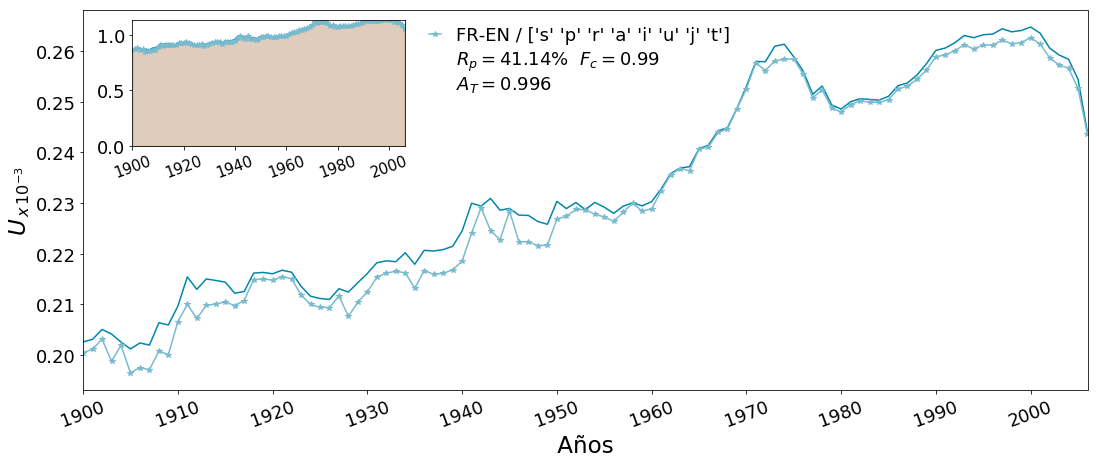
\includegraphics[scale=.375]{OM_1.png}
	\caption{Eliminación de palabras del francés en el inglés. A pesar de eliminar el 40$\%$ de las palabras del francés en el inglés, año con año el uso reducido es próximo al original, y en algunos años iguales, resultando en una mayor similitud  entre ambos conjuntos al ser el área de traslape de 0.996.}
	\label{fig.OM1}
\end{figure}


\begin{figure}[]
	\centering
	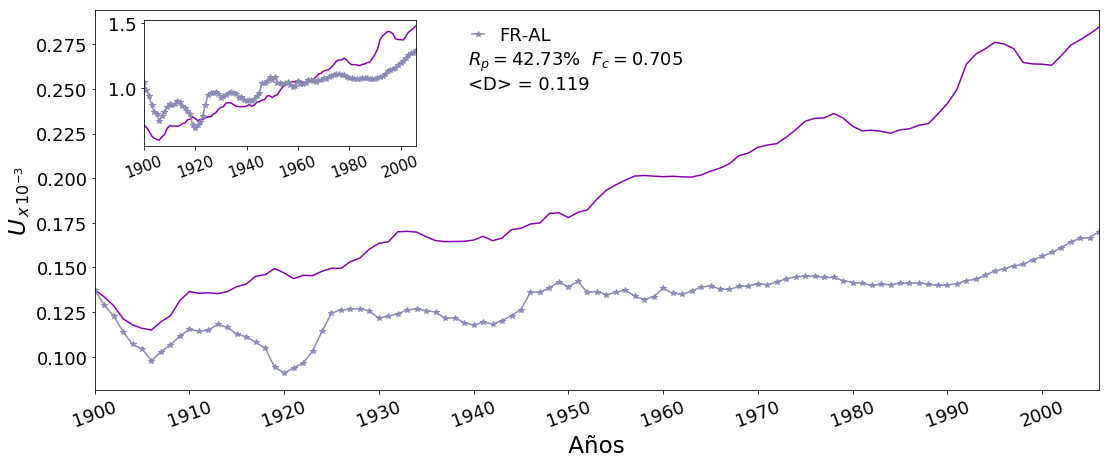
\includegraphics[scale=.375]{OM_2.png}
	\caption{Eliminación de palabras del francés en el italiano. Tras eliminar casi el 50$\%$ de las palabras del francés en el italiano, el uso en ambos conjuntos obtuvo una buena similitud de 0.946, a pesar de que cada valor del uso reducido sea en promedio la mitad de su correspondiente en el uso original.}
	\label{fig.OM2}
\end{figure}

\begin{figure}[]
	\centering
	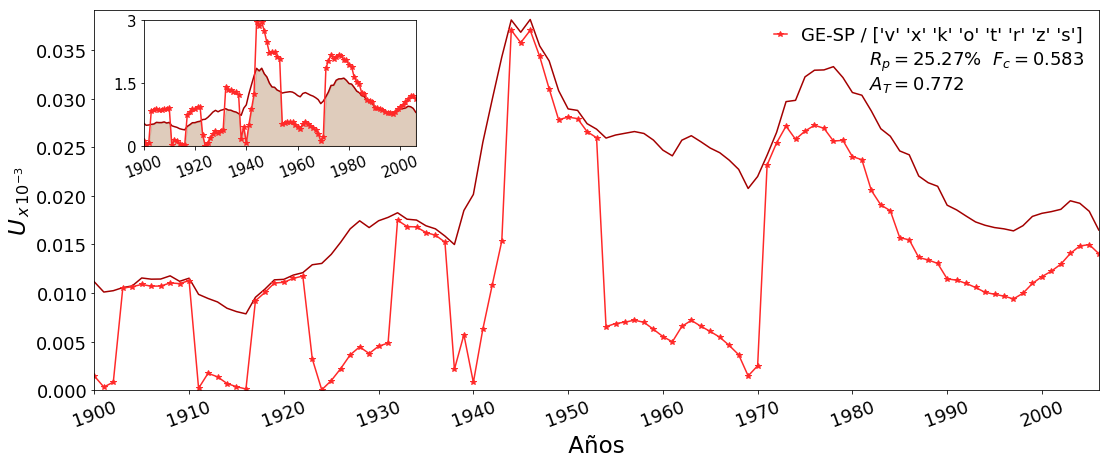
\includegraphics[scale=.375]{OM_3.png}
	\caption{Eliminación de palabras del alemán en el español. Tras eliminar el 40$\%$ de las palabras del alemán en el español, y  tener en algunos años el uso reducido y el uso original valores próximos entre si, no hay una similitud en ambos conjuntos al ser el area de traslape de 0.772}
	\label{fig.OM3}
\end{figure}






De las figuras~\ref{fig.OM1} y~\ref{fig.OM2}, se puede ver que a pesar de tener valores similares del porcentaje de reducción, el factor de conversión es diferente en cada caso. Por lo que el factor de conversión es independiente de la cantidad de palabras que se eliminen (porcentaje de reducción), y ambos valores no influyen en el área de traslape, ya que en las dos graficas el área de traslape es mayor a 0.9. 

Con la figura~\ref{fig.OM3} también se muestra la conclusión anterior. En este caso, a pesar de que se elimino una menor cantidad de palabras, el área de traslape es la peor entre las tres graficas, no obstante el factor de conversión es similar al de la figura~\ref{fig.OM2}.


\section{Resultados generales}

El realizar diferentes elecciones para reducir la cantidad de palabras migrantes, mostró que los posibles errores en la clasificación de los datos, no modifican (en la mayoría de los casos) los resultados obtenidos sobre el uso de un idioma en otro. Sin embargo en el caso de los préstamos nuevos, al mostrar relevancia el significado de las palabras, una posible limpieza podría eliminar palabras de determinados campos semánticos, lo cual llevaría a una perdida de la información. 

También se destaca al uso de un idioma en otro, como una propiedad común para cada pareja de idiomas, donde no tiene tanta relevancia la cantidad de palabras que conformen los préstamos acumulados,  en conjunto, todas ellas se comportarán de la misma manera. 

%El proceso de relacionar las palabras migrantes con campos semánticos y eventos históricos que justifiquen su aparición, permitió establecer un forma para cuantificar la influencia entre idiomas llamada uso. Todo este método se facilitó por la eliminación de las palabras funcionales, dejando sólo palabras de contenido, pero ¿cómo se modificaría el uso entre idiomas si se eliminaran otro tipo de palabras, sin importar si estás son de contenido?

%Para responder esta pregunta, se ha elaborado un nuevo algoritmo que reduce el conjunto de las palabras migrantes, y  obtiene nuevos valores para el uso entre idiomas.  Elegidos una pareja de idioma origen \textit{A} e idioma receptor \textit{B}, el proceso es el siguiente. 


%\jmnote{corregir "verdadero" en el parrafo}
%Si el uso en el conjunto original se toma como verdadero (ya que con el se obtuvieron los resultados del capítulo anterior), una forma de determinar que tanto cambió el uso en el conjunto reducido, es a partir del coeficiente de determinación $R^{2}$. 

%Si para un año $t$ dentro de un intervalo de tiempo $\Delta t$,  se detonan como $O_{t}$ al uso en el conjunto original y $v_{t}$ al uso en el al uso en el conjunto reducido,  mientras que $\bar{v}$ es el promedio de todos los $v_{t}$ en el intervalo, entonces el coeficiente de determinación se expresa como: 
%Para un año $t$ dentro de un intervalo de tiempo,  el uso en el conjunto original y el uso en el conjunto reducido se detonan como $O_{t}$ y $v_{t}$ respectivamente,  mientras que $\bar{v}$ es el promedio de todos los $v_{t}$ en el intervalo, entonces el coeficiente de determinación queda definido como: 
%\begin{equation}
%\label{ec.dif_uso}
%R^{2} = 1 - \sum_{t} \frac{ \left( v_{t}- O_{t} \right)^{2}  }{ \left( v_{t} - \bar{v} \right)^{2} }.
%\end{equation}
%Se empleará el concepto \textbf{conservación del uso} para aquellos idiomas cuyo uso no cambie en un intervalo de tiempo. La conservación es favorable si $R^{2}$ es próximo a 1. 
%Si la conservación no es favorable, las palabras eliminadas son las más relevantes para las migraciones de \textit{A} en \textit{B}.


%La conservación del uso y sus características no siempre serán la mismas tras una eliminación con diferentes letras, sin embargo, es posible decir con los datos de las cien mil eliminaciones, si el uso se conserva.  Para ello, se agruparon y promediaron por cada idioma origen  los valores del coeficiente de determinación, obteniendo un $\left \langle R^{2}  \right \rangle$  promedio con el cual decir de manera general, si el uso del idioma origen se conserva. 

%La tabla~\ref{tab.conservacion} muestra por cada idioma origen,  el valor de $\left \langle R^{2}  \right \rangle$ correspondiente, así como  en cuales idiomas receptores el promedio de $R^{2}$ fue mayor, y en cuales el promedio $R^{2}$ fue menor. De esta tabla se puede ver que el alemán es el idioma con los valores más bajos de $R^{2}$, donde la menor conservación se dio con el español. Los demás idiomas tienen valores aceptables con los cuales decir que su uso se conserva a pesar de las eliminaciones. 

%Como la intención de las eliminaciones es simular reglas que limpien los datos, se puede decir que los préstamos con más errores son los del alemán en el español, ya que si se hubiese tal criterio, los resultados de esta pareja serian los más afectados. En los demás idiomas no habría un cambio significativo. 

%De esta tabla se puede ver que la conservación del uso es menor, en las combinaciones donde el alemán este presente, ya sea como idioma origen o como idioma receptor. No obstante, en los demás idiomas la conservación del uso fue favorable, por lo que se puede decir que los idiomas conservan su uso, sin importar  cuales sean las palabras que conformen a las migraciones. 

%Con estos resultados se puede decir que el uso entre idiomas, no es afectado por reducir la cantidad de palabras que conforman a las migraciones,   


%\begin{table}
%	\centering
%	\begin{tabular}{cccc}
%		\textbf{} & \textbf{$\left \langle R^{2} \right \rangle$} & \textbf{$R^{2}_{max}$} & \textbf{$R^{2}_{min}$} \\
%		\textbf{inglés}   & 0.85 $\pm$ 0.14   &  IT 0.97 $\pm$ 0.01  & GE 0.77 $\pm$ 0.03  \\
%		\textbf{francés}  & 0.83 $\pm$ 0.12   &  EN 0.95 $\pm$ 0.02  & GE 0.66 $\pm$ 0.02  \\
%		\textbf{alemán}   & 0.75 $\pm$ 0.06   &  EN 0.80 $\pm$ 0.06  & SP 0.51 $\pm$ 0.33  \\
%		\textbf{italiano} & 0.87 $\pm$ 0.14   &  FR 0.93 $\pm$ 0.08  & GE 0.68 $\pm$ 0.03  \\
%		\textbf{español}  & 0.88 $\pm$ 0.05   &  IT 0.94 $\pm$ 0.06  & GE 0.71 $\pm$ 0.01                                                               
%	\end{tabular}
%	\caption{Conservación del uso de los idiomas. El español es el idioma que es menos afectado por las eliminaciones y que conserva más su uso en los demás, seguido del italiano, el inglés, el francés y por ultimo el alemán.}
%	\label{tab.conservacion}
%\end{table}



%El tratar a las migraciones de palabras como un conjunto, donde no tiene tanta relevancia las palabras que lo conforman, muestra propiedades estadísticas comunes que cumplen las parejas de idiomas. Por el momento  

   
%Individualmente. los valores de uso de una única palabra pueden ser distintos a los de otra palabra, sin embargo al tratar a todo el conjunto, el uso se comporta de la misma manera, sin importar los valores individuales de los elementos que lo conforman. 

%A pesar de haber errores en el algoritmo que clasifica tanto a los idiomas orígenes, como a sus  palabras migrantes, la conservacion del uso puede justificar que no importa si se eliminan las palabras mal clasificadas, en términos numéricos, el uso de un idioma otro va a ser el mismo.  

